\documentclass[showpacs, preprintnumbers, pra, superscriptaddress, floatfix, onecolumn, longbibliography]{revtex4-1}
\usepackage{amssymb}
\usepackage{amsmath}
\usepackage{float}
\usepackage{graphicx}
\usepackage{epsfig}
\usepackage[T1]{fontenc}
\usepackage{color}


\usepackage[utf8]{inputenc}
%\topmargin=0.2cm

\newcommand{\beq}{\begin{equation}}
\newcommand{\eeq}{\end{equation}}
\newcommand{\bea}{\begin{eqnarray}}
\newcommand{\eea}{\end{eqnarray}}
\newcommand{\nn}{\nonumber}
\newcommand{\no}{\noindent}
\newcommand{\hs}{\hspace{0.1cm}}
\newcommand{\spz}{\hspace{0.7cm}}
\newcommand{\st}{\stackrel}
\newcommand{\eps}{\epsilon}
\newcommand{\veps}{\varepsilon}
\newcommand{\al}{\alpha}
\newcommand{\s}{\sigma}
\newcommand{\lam}{\lambda}
\newcommand{\om}{\omega}
\newcommand{\iom}{i\omega_n}
\newcommand{\de}{\delta}
\newcommand{\D}{\Delta}
\newcommand{\goto}{\rightarrow}
\newcommand{\lab}{\label}
\newcommand{\be}{\beta}
\newcommand{\zb}{\bar{z}}
\newcommand{\p}{\partial}\newcommand{\vp}{\varphi}
\newcommand{\ra}{\rangle}
\newcommand{\la}{\langle}
\newcommand{\Ga}{\Gamma}
\newcommand{\ga}{\gamma}
\newcommand{\app}{\approx}
\newcommand{\ua}{\uparrow}
\newcommand{\da}{\downarrow}
\newcommand{\Ua}{\Uparrow}
\newcommand{\Da}{\Downarrow}
\newcommand{\dmi}{\frac{1}{2}}
\newcommand{\lra}{\longrightarrow}
\newcommand{\Lra}{\Leftrightarrow}
\newcommand{\tht}{\theta}
\newcommand{\pbf}{}
\newcommand{\SM}{S}
\newcommand{\uul}[1] {\underline{\underline{ #1}}}
\def\mean#1{\left< #1 \right>}

\begin{document}

\title{}


\maketitle

\section{Details of the density-functional calculations}

The structural model used in the density-functional calculations (DFT) consists of four MnBi$_4$Te$_7$ unit cells and of a vacuum of 30 Bohr radii (Fig. \ref{dft_structure}a). We use the experimental bulk lattice parameters and atomic positions.
The calculations are based on the GGA+U method with the generalized grandient approximation \cite{perdew1996generalized} as implemented in the FPLO code version 48.00-52 \cite{PhysRevB.59.1743}. We fix parameters $U=5.34\,$eV and $J=0$, as in Ref. \cite{otrokov2019prediction} and use the atomic limit flavor for the double counting correction. The spin-orbit interaction is considered in the fully-relativistic four-component formalism. Numerial k-space integrations are performed with a tetrahedron method with a mesh of $12\times12\times1$ subdivisions in the Brillouin zone. For the calculations of the density of states (DOS), we consider a mesh of $30\times30\times1$ subdivisions.

For the simulation of the orbital-projected surface spectral density in Fig. 3 of the main text, we take into account all Bloch states in the slab, weighting their contribution with an exponentially decaying factor (Fig. \ref{dft_structure}b). Specifically, denoting the local orbitals as $|\phi^{(z)}_{jm}\rangle$, where $z$ is the distance from the orbital center to the surface, for each Bloch state $|\psi_{k_0\nu}\rangle$ of energy $\varepsilon_{k_0\nu}$, we consider as its contribution 
\begin{equation}
A^{k_0,\nu}_{jm}(\omega,k)=\frac{1}{\pi}\frac{ \Delta_\varepsilon}{(\omega-\varepsilon_{k_0\nu})^2 + \Delta^2_\varepsilon}\frac{ \Delta_k}{(k-k_0)^2 + \Delta^2_k }|\langle \phi^{(z)}_{jm} | \psi_{k_0\nu} \rangle|^2 \text{e}^{-z/\lambda},
\end{equation}
where $\lambda=10\,$\AA, $\Delta_\varepsilon=20\,$meV and $\Delta_k=0.005$\AA$^{-1}$. Last, notice that the local orbitals in Fig. 3 of the main text are defined with the cartesian coordinate system shown in Fig. \ref{dft_structure}c).

\begin{figure*}[h!]
 \centering
 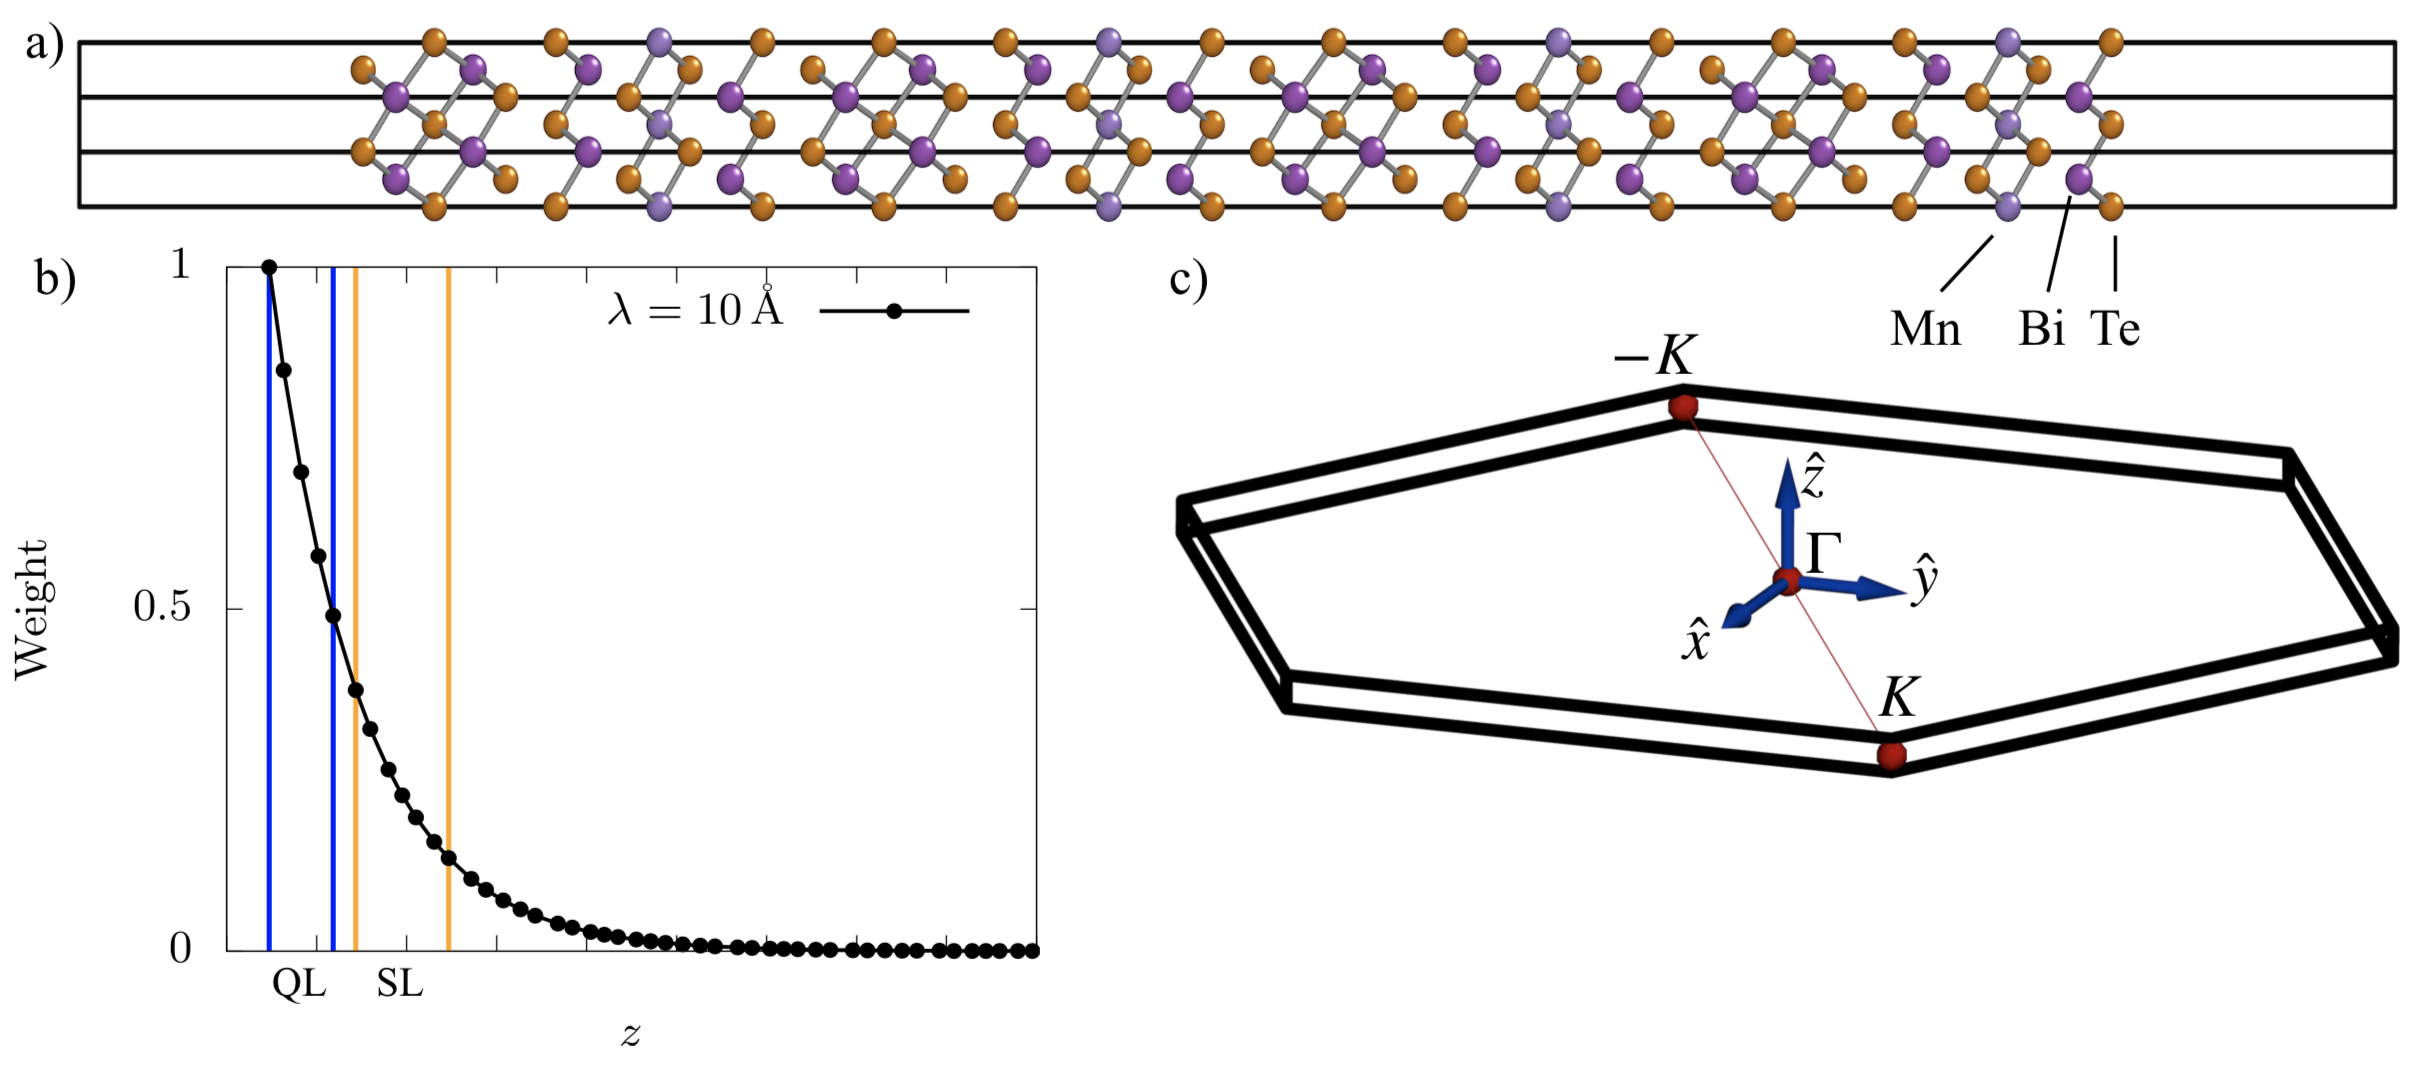
\includegraphics[width=14 cm]{structural_data.png}
	\caption{a) Structural model used in the density-functional calculation. b) Illustration of the exponential decaying weight considered for the surface spectral weight simulation. c) Brillouin zone.} 
	\label{dft_structure}
\end{figure*}

\section{Surface DOS}

Fig. \ref{dft_dos} shows the orbital-projected DOS corresponding to different parts of the slab. Specifically, we consider the projection of the total DOS on the inner-most unit-cell as representative of the bulk, while for the surface DOS we sum the local DOS of all of the atoms in the slab weighted by a function that  exponentially decays from the corresponding surface.
While Bi-$6p$ and Te-$5p$ in all cases provide the leading contributions, the different electronic structure at the two terminations reflects in the apperance of stronger hybridization effects for the surface with quintuple layer termination.

\begin{figure*}[h!]
 \centering
 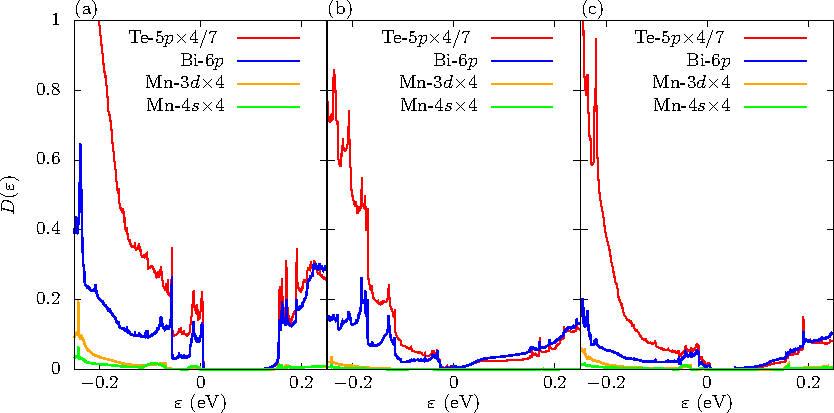
\includegraphics[width=15 cm]{dos.pdf}
	\caption{ Bulk DOS (a) and surface DOS for the quintuple layer (b) and septuple layer (c) terminations. For the bulk DOS, we consider the total DOS of the slab projected on the quintuple and septuple layer in the center of the slab.  For the surface DOS, we sum the local DOS of all the atoms in the slab, weighted by an exponential decay from the corresponding surface. Notice that the Mn and the Te contribution have been scaled by 4 and 4/7, respectively.	
}
	\label{dft_dos}
\end{figure*}



\section{Surface state angular momentum reversal within DFT}
Fig. \ref{dft_sl} illustrates the angular momentum reversal between the upper and lower parts of the surface state, as obtained with DFT. 
Fig. \ref{dft_sl}a) presents the band-structure projected on the outmost septuple layer and Fig. \ref{dft_sl}b) shows constant-energy contours. The color-scale reflects the amplitude of the corresponding states projected on local orbitals of Bi or Te and $J=1/2$, which we found dominate the upper part of the Dirac cone.
Notice that, since the experiment of natural dichroism described in the main text is essentially susceptible to the in-plane angular momentum, in this figure the fully relativistic local orbitals considered are defined with the quantization axis along the in-plane cartesian direction $\hat{x}$.
\begin{figure*}[h!]
 \centering
 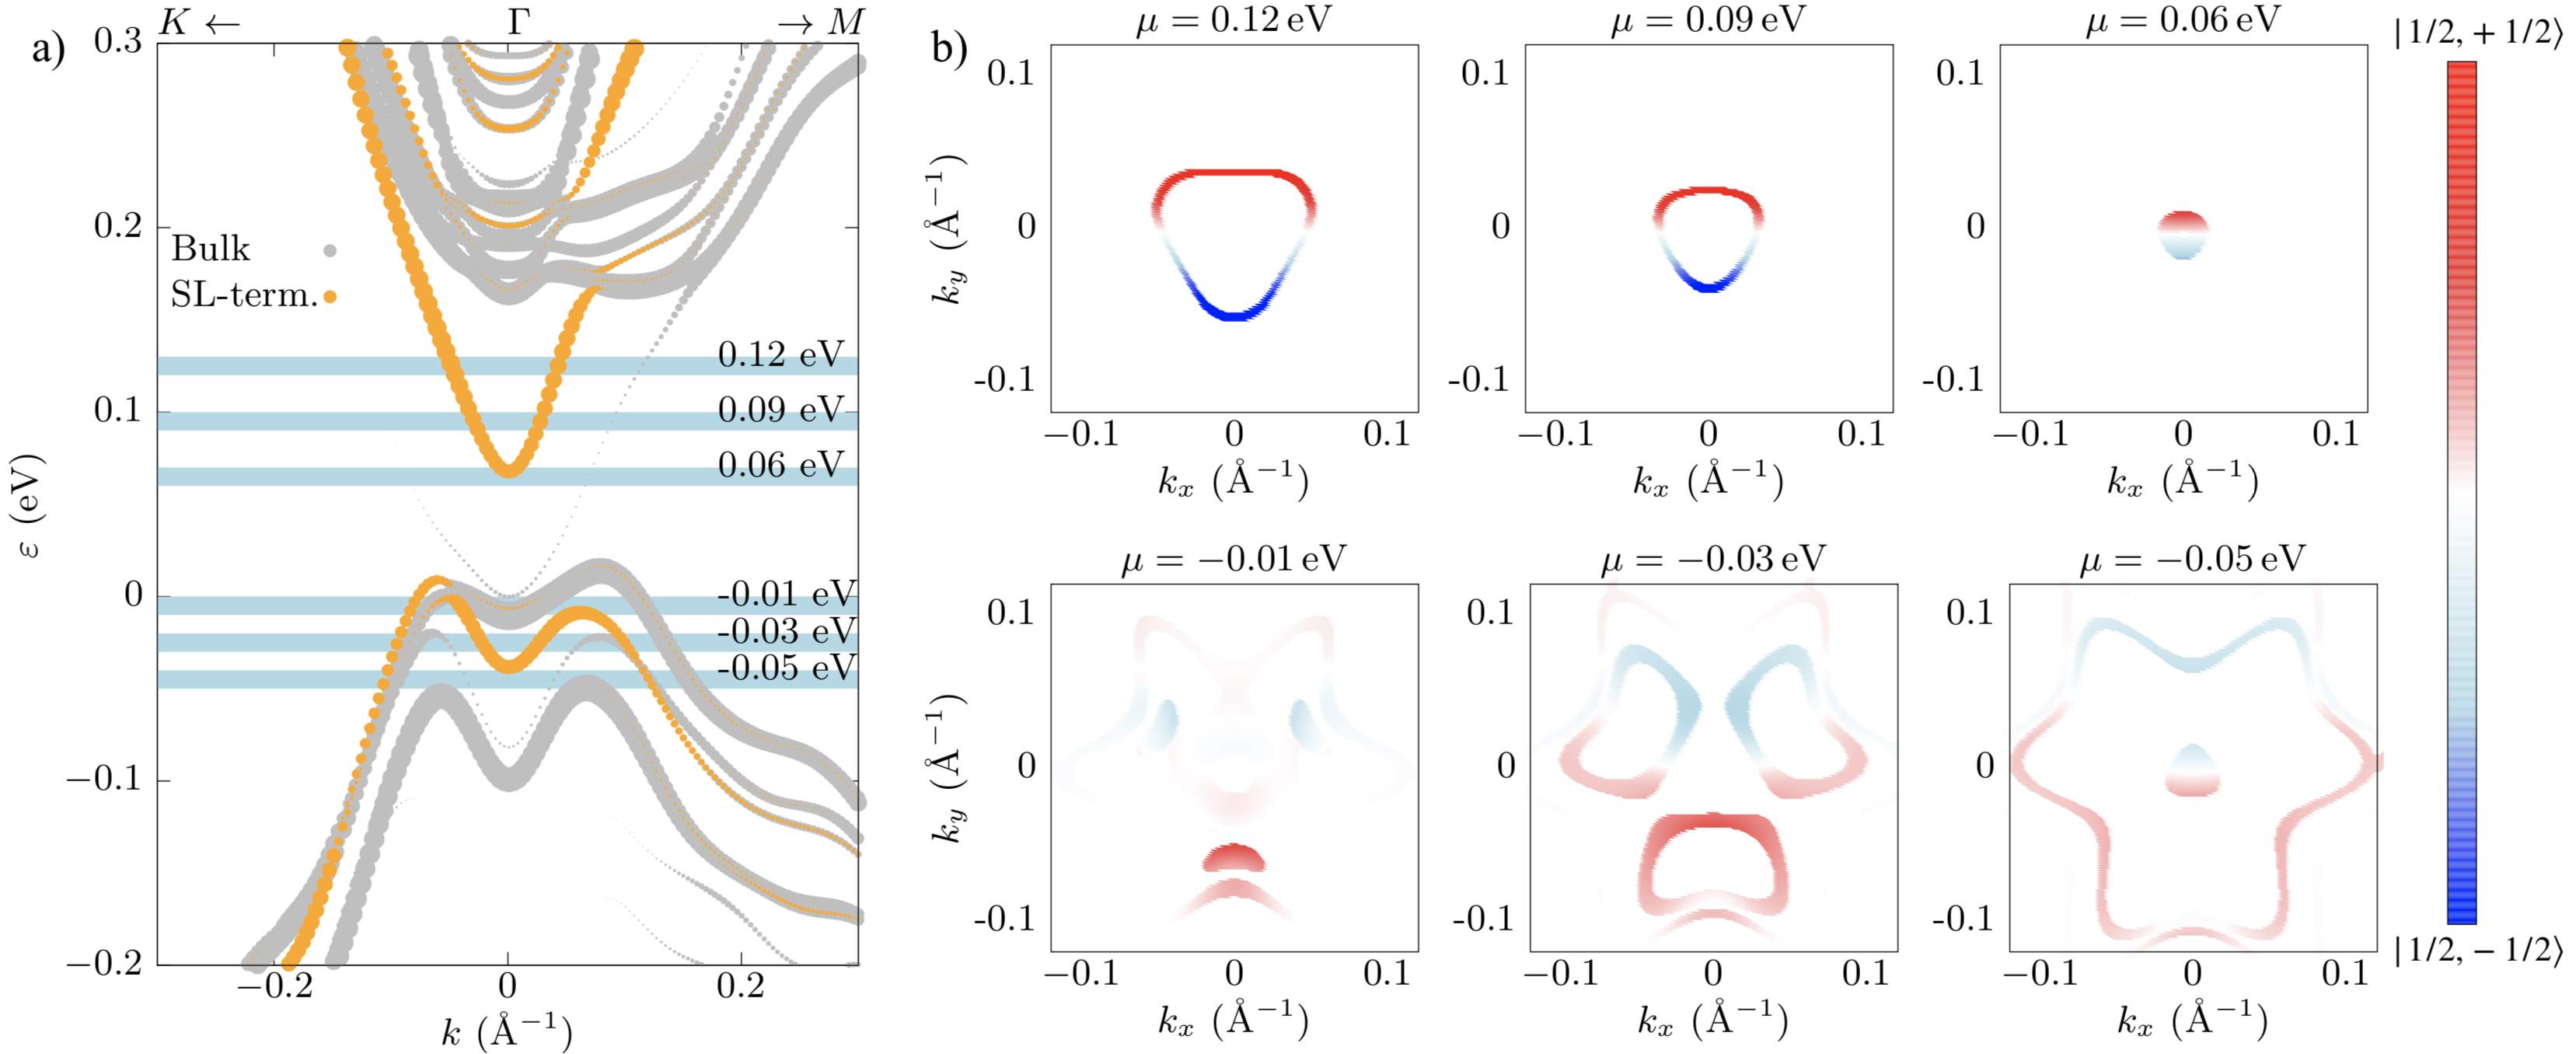
\includegraphics[width=18 cm]{sl.png}
	\caption{a) MnBi$_4$Te$_7$ band structure projected on the outmost septuple layer (SL-term.) and on the four inner blocks (Bulk). 
	b): Constant energy contours of septuple layer-projected band-structure. In this projection, for simplicity we only consider the Bi or Te states with $J=1/2$, which we found to dominate the upper part of the Dirac cone.
	}
	\label{dft_sl}
\end{figure*}


\bibliography{ref}
\end{document}


